\section{Exercices ludiques}

\exo{pyramide} Compléter les pyramides suivantes de sorte à ce que chaque case soit égale à la somme des deux cases du dessous. Ecrire les résultats en heures, minutes et secondes.

\begin{minipage}[t]{0.45\textwidth}
	\begin{center}
	\begin{tikzpicture}[scale=1.05]
 		\foreach \j [count=\xi]  in { }
 				{\draw (-3+2*\xi,0) rectangle (-1+2*\xi,1);
 				\node at (-2+2*\xi,0.5) {\j};}
 		\foreach \j [count=\xi]  in { ,  }
 				{\draw (-4+2*\xi,-1) rectangle (-2+2*\xi,0);
 				\node at (-3+2*\xi,-0.5) {\j};}
 		\foreach \j [count=\xi]  in { ,  , 2min 05s}
 				{\draw (-5+2*\xi,-2) rectangle (-3+2*\xi,-1);
 				\node at (-4+2*\xi,-1.5) {\j};}
 		\foreach \j [count=\xi]  in {1min 22s, 41s, 37s, }
 				{\draw (-6+2*\xi,-3) rectangle (-4+2*\xi,-2);
 				\node at (-5+2*\xi,-2.5) {\j};}
\end{tikzpicture}
	\end{center}

\end{minipage}
\hfil
\vrule
\hfil
\begin{minipage}[t]{0.45\textwidth}
	\begin{center}
	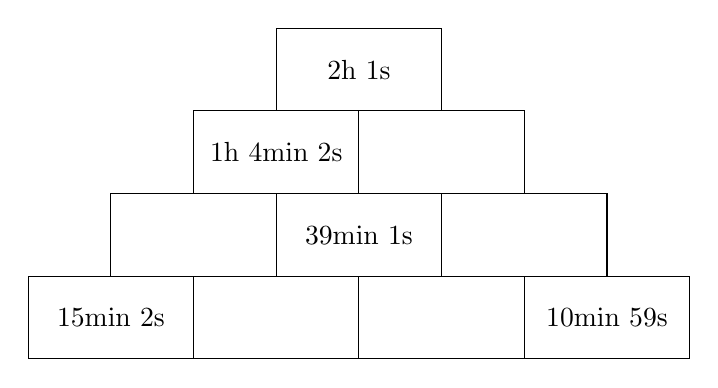
\begin{tikzpicture}[scale=1.05]
 		\foreach \j [count=\xi]  in {2h 1s}
 				{\draw (-3+2*\xi,0) rectangle (-1+2*\xi,1);
 				\node at (-2+2*\xi,0.5) {\j};}
 		\foreach \j [count=\xi]  in {1h 4min 2s,  }
 				{\draw (-4+2*\xi,-1) rectangle (-2+2*\xi,0);
 				\node at (-3+2*\xi,-0.5) {\j};}
 		\foreach \j [count=\xi]  in { , 39min 1s,  }
 				{\draw (-5+2*\xi,-2) rectangle (-3+2*\xi,-1);
 				\node at (-4+2*\xi,-1.5) {\j};}
 		\foreach \j [count=\xi]  in {15min 2s,  ,  , 10min 59s}
 				{\draw (-6+2*\xi,-3) rectangle (-4+2*\xi,-2);
 				\node at (-5+2*\xi,-2.5) {\j};}
\end{tikzpicture}
	\end{center}

\end{minipage}

\newpage 

\exo{sudoku} Compléter les grilles de Sudoku suivantes en inscrivant les restes des divisions euclidiennes dans les cases données, puis à l'aide des règles classiques de Sudoku.
\vfil
\setlength{\columnseprule}{0pt}\begin{minipage}{0.55\textwidth}
\begin{center}
	 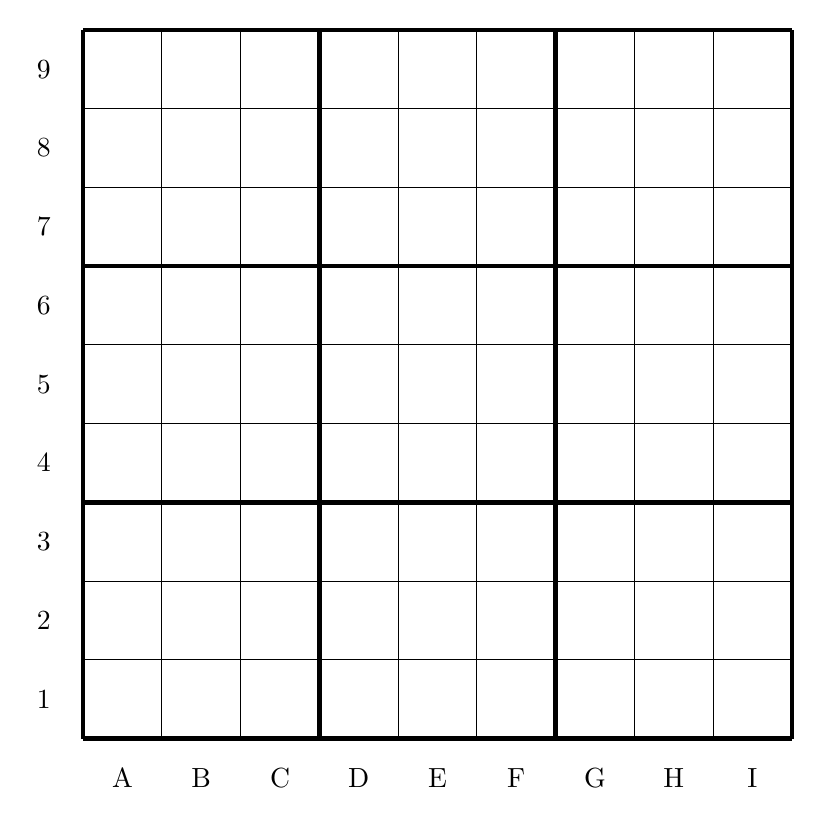
\begin{tikzpicture}
		 \draw[thin] (0,0) grid (9,9);
		 \draw[ultra thick,step=3] (0,0) grid (9,9);
		 \foreach \x/\y in {1/A,2/B,3/C,4/D,5/E,6/F,7/G,8/H,9/I}
			 { \draw node at (\x-0.5,-0.5) {\y};
			 \draw node at (-0.5,\x-0.5) {\x}; }
		 \end{tikzpicture}	
	 \end{center}
\end{minipage}
\hfil\vrule\hfil
\begin{minipage}{0.4\textwidth}
\begin{itemize}[leftmargin=10pt]\begin{multicols}{2}
\item(A;9) : 90852\div11

\item(C;9) : 9973\div4

\item(E;9) : 92801\div11

\item(G;9) : 77785\div9

\item(I;9) : 36210\div11

\item(B;8) : 20999\div5

\item(D;8) : 27668\div11

\item(F;8) : 17015\div11

\item(H;8) : 61485\div11

\item(A;7) : 5815\div8

\item(C;7) : 29049\div10

\item(E;7) : 65092\div7

\item(G;7) : 26218\div5

\item(I;7) : 42106\div6

\item(B;6) : 797\div6

\item(H;6) : 34432\div6

\item(A;5) : 64316\div10

\item(C;5) : 9573\div11

\item(E;5) : 36412\div6

\item(G;5) : 34659\div10

\item(I;5) : 23115\div7

\item(B;4) : 29140\div11

\item(H;4) : 2399\div8

\item(A;3) : 17225\div7

\item(C;3) : 24972\div8

\item(E;3) : 13105\div9

\item(G;3) : 48487\div5

\item(I;3) : 17056\div11

\item(B;2) : 39697\div11

\item(D;2) : 32734\div6

\item(F;2) : 78438\div8

\item(H;2) : 14640\div7

\item(A;1) : 57690\div8

\item(C;1) : 106794\div11

\item(E;1) : 74330\div9

\item(G;1) : 27472\div6

\item(I;1) : 37583\div8

\item[\vspace{\fill}]\end{multicols}\end{itemize}\end{minipage}
\vfil
\setlength{\columnseprule}{0pt}\begin{minipage}{0.55\textwidth}
\begin{center}
	 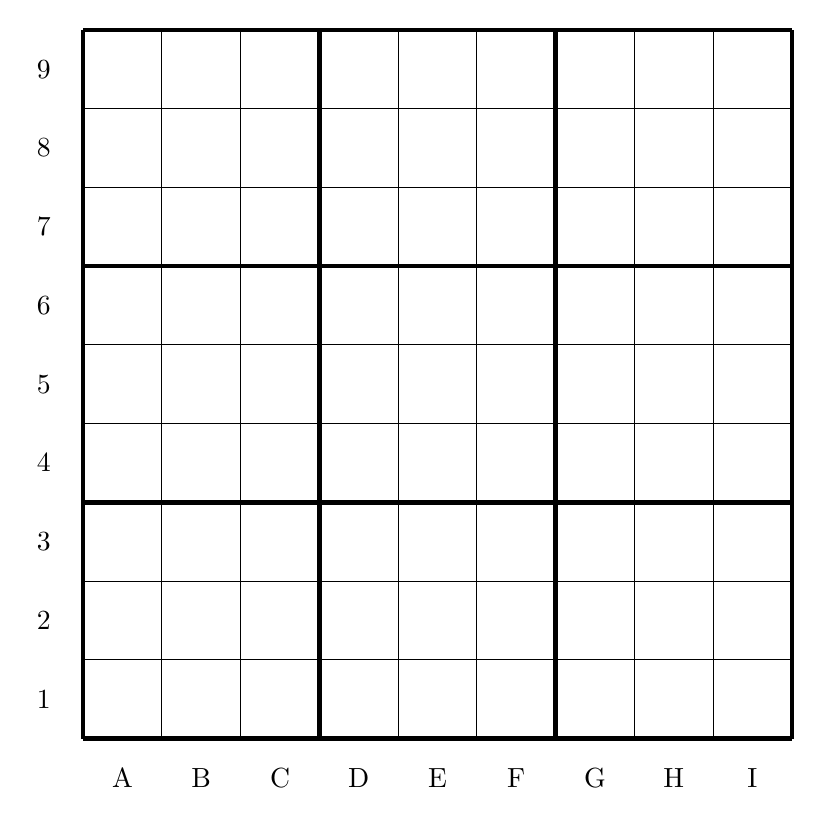
\begin{tikzpicture}
		 \draw[thin] (0,0) grid (9,9);
		 \draw[ultra thick,step=3] (0,0) grid (9,9);
		 \foreach \x/\y in {1/A,2/B,3/C,4/D,5/E,6/F,7/G,8/H,9/I}
			 { \draw node at (\x-0.5,-0.5) {\y};
			 \draw node at (-0.5,\x-0.5) {\x}; }
		 \end{tikzpicture}	
	 \end{center}
\end{minipage}
\hfil\vrule\hfil
\begin{minipage}{0.4\textwidth}
\begin{itemize}[leftmargin=10pt]\begin{multicols}{2}
\item(A;9) : 5233\div11

\item(E;9) : 54031\div7

\item(I;9) : 89950\div9

\item(B;8) : 41073\div6

\item(D;8) : 29901\div7

\item(E;8) : 19680\div11

\item(F;8) : 52442\div10

\item(H;8) : 2556\div15

\item(C;7) : 104077\div15

\item(G;7) : 55172\div18

\item(D;6) : 143271\div18

\item(A;5) : 8518\div8

\item(B;5) : 57704\div10

\item(E;5) : 144316\div17

\item(H;5) : 66239\div7

\item(I;5) : 128067\div14

\item(F;4) : 40497\div8

\item(C;3) : 152172\div17

\item(G;3) : 155891\div16

\item(B;2) : 179197\div19

\item(D;2) : 115441\div13

\item(E;2) : 15562\div17

\item(F;2) : 8572\div13

\item(H;2) : 14185\div16

\item(A;1) : 79583\div11

\item(E;1) : 139998\div19

\item(I;1) : 50531\div11

\item[\vspace{\fill}]\end{multicols}\end{itemize}\end{minipage}

\newpage
\input{Exercices_Contenu/PixelArt1.tex}

\exo{Labyrinthe1} Traverser le labyrinthe en franchissant les cases dans l'ordre croissant 

\begin{center}
\tikzmath{\sizex = 7 ;\sizexm=\sizex-1 ; \sizey=7 ; \sizeym=\sizey-1;}
\begin{tikzpicture}[scale=1.5]
	\foreach \i in {0,...,\sizex}
 		{\foreach \j in {0,...,\sizey}
 			{\draw ({max(\i-0.2,0)},\j)--({min(\sizex,\i+0.2)},\j);
			\draw (\i,{max(0,\j-0.2)})--(\i,{min(\sizey,\j+0.2)}); }}
	\draw (0,0) rectangle (\sizex,\sizey) ;
	\draw[thick,white] (0,\sizey-0.1)--(0,\sizeym+0.2) ;
 	\draw[thick,white] (\sizex,0.2)--(\sizex,0.8) ;
	\draw[-{Latex[length=3mm,width=5mm]}] (-0.5,\sizey-0.5)--(0,\sizey-0.5) ;
	\draw[-{Latex[length=3mm,width=5mm]}] (\sizex,0.5)--(\sizex+0.5,0.5) ;
	\node at (0.5,6.5) {92s};
	\node at (1.5,6.5) {1.23min};
	\node at (2.5,6.5) {245s};
	\node at (3.5,6.5) {3.95min};
	\node at (4.5,6.5) {272s};
	\node at (5.5,6.5) {4.81min};
	\node at (6.5,6.5) {291s};
	\node at (0.5,5.5) {1.56min};
	\node at (1.5,5.5) {74s};
	\node at (2.5,5.5) {4.16min};
	\node at (3.5,5.5) {259s};
	\node at (4.5,5.5) {4.4min};
	\node at (5.5,5.5) {248s};
	\node at (6.5,5.5) {5.18min};
	\node at (0.5,4.5) {98s};
	\node at (1.5,4.5) {1.48min};
	\node at (2.5,4.5) {238s};
	\node at (3.5,4.5) {3.76min};
	\node at (4.5,4.5) {262s};
	\node at (5.5,4.5) {5.6min};
	\node at (6.5,4.5) {323s};
	\node at (0.5,3.5) {2.0min};
	\node at (1.5,3.5) {100s};
	\node at (2.5,3.5) {3.93min};
	\node at (3.5,3.5) {228s};
	\node at (4.5,3.5) {3.45min};
	\node at (5.5,3.5) {350s};
	\node at (6.5,3.5) {5.21min};
	\node at (0.5,2.5) {137s};
	\node at (1.5,2.5) {2.63min};
	\node at (2.5,2.5) {142s};
	\node at (3.5,2.5) {3.76min};
	\node at (4.5,2.5) {216s};
	\node at (5.5,2.5) {6.1min};
	\node at (6.5,2.5) {347s};
	\node at (0.5,1.5) {1.9min};
	\node at (1.5,1.5) {176s};
	\node at (2.5,1.5) {3.3min};
	\node at (3.5,1.5) {204s};
	\node at (4.5,1.5) {3.03min};
	\node at (5.5,1.5) {380s};
	\node at (6.5,1.5) {6.7min};
	\node at (0.5,0.5) {93s};
	\node at (1.5,0.5) {2.55min};
	\node at (2.5,0.5) {187s};
	\node at (3.5,0.5) {3.06min};
	\node at (4.5,0.5) {177s};
	\node at (5.5,0.5) {6.13min};
	\node at (6.5,0.5) {412s};
\end{tikzpicture}
\end{center}

\newpage
\exo{PixelArt2}Colorie en noir uniquement les nombres qui ne sont pas premiers.

\begin{figure}[H]
\center
\begin{tikzpicture}[scale=1.3]
\newcommand{\y}{0}\renewcommand{\y}{0}
\foreach \x [count=\xi] in {2, 3, 5, 4, 6, 9, 10, 15, 7, 11, 13, 17}
{\draw (\xi,\y) rectangle (\xi +1,\y -1) node[pos=0.5]{{ \x}};}
\renewcommand{\y}{-1}
\foreach \x [count=\xi] in {19, 23, 18, 29, 31, 37, 21, 41, 43, 47, 53, 59}
{\draw (\xi,\y) rectangle (\xi +1,\y -1) node[pos=0.5]{{ \x}};}
\renewcommand{\y}{-2}
\foreach \x [count=\xi] in {61, 25, 67, 71, 27, 33, 35, 39, 42, 73, 79, 83}
{\draw (\xi,\y) rectangle (\xi +1,\y -1) node[pos=0.5]{{ \x}};}
\renewcommand{\y}{-3}
\foreach \x [count=\xi] in {89, 45, 97, 49, 51, 55, 57, 60, 63, 72, 101, 103}
{\draw (\xi,\y) rectangle (\xi +1,\y -1) node[pos=0.5]{{ \x}};}
\renewcommand{\y}{-4}
\foreach \x [count=\xi] in {75, 107, 109, 78, 81, 85, 91, 99, 102, 105, 113, 127}
{\draw (\xi,\y) rectangle (\xi +1,\y -1) node[pos=0.5]{{ \x}};}
\renewcommand{\y}{-5}
\foreach \x [count=\xi] in {131, 137, 139, 111, 119, 151, 149, 157, 163, 167, 173, 179}
{\draw (\xi,\y) rectangle (\xi +1,\y -1) node[pos=0.5]{{ \x}};}
\renewcommand{\y}{-6}
\foreach \x [count=\xi] in {181, 191, 193, 121, 132, 197, 134, 144, 199, 155, 211, 223}
{\draw (\xi,\y) rectangle (\xi +1,\y -1) node[pos=0.5]{{ \x}};}
\renewcommand{\y}{-7}
\foreach \x [count=\xi] in {227, 229, 233, 239, 241, 251, 158, 160, 257, 165, 263, 171}
{\draw (\xi,\y) rectangle (\xi +1,\y -1) node[pos=0.5]{{ \x}};}
\renewcommand{\y}{-8}
\foreach \x [count=\xi] in {180, 185, 190, 192, 200, 269, 271, 277, 281, 283, 293, 183}
{\draw (\xi,\y) rectangle (\xi +1,\y -1) node[pos=0.5]{{ \x}};}
\renewcommand{\y}{-9}
\foreach \x [count=\xi] in {187, 307, 311, 313, 189, 317, 195, 192, 207, 209, 331, 337}
{\draw (\xi,\y) rectangle (\xi +1,\y -1) node[pos=0.5]{{ \x}};}
\renewcommand{\y}{-10}
\foreach \x [count=\xi] in {221, 347, 225, 349, 230, 353, 359, 231, 237, 367, 373, 240}
{\draw (\xi,\y) rectangle (\xi +1,\y -1) node[pos=0.5]{{ \x}};}
\renewcommand{\y}{-11}
\foreach \x [count=\xi] in {245, 379, 255, 383, 258, 389, 397, 401, 409, 419, 421, 267}
{\draw (\xi,\y) rectangle (\xi +1,\y -1) node[pos=0.5]{{ \x}};}
\renewcommand{\y}{-12}
\foreach \x [count=\xi] in {270, 431, 273, 433, 285, 439, 291, 299, 301, 305, 443, 310}
{\draw (\xi,\y) rectangle (\xi +1,\y -1) node[pos=0.5]{{ \x}};}
\renewcommand{\y}{-13}
\foreach \x [count=\xi] in {315, 449, 457, 461, 321, 463, 467, 479, 487, 491, 499, 503}
{\draw (\xi,\y) rectangle (\xi +1,\y -1) node[pos=0.5]{{ \x}};}
\renewcommand{\y}{-14}
\foreach \x [count=\xi] in {324, 330, 345, 343, 351, 509, 521, 523, 541, 355, 547, 557}
{\draw (\xi,\y) rectangle (\xi +1,\y -1) node[pos=0.5]{{ \x}};}
\end{tikzpicture}
\end{figure}

\newpage
\exo{Labyrinthe2} Traverser le labyrinthe en franchissant les cases dans l'ordre décroissant 

\begin{center}
\tikzmath{\sizex = 9 ;\sizexm=\sizex-1 ; \sizey=10 ; \sizeym=\sizey-1;}
\begin{tikzpicture}[scale=1.7]
	\foreach \i in {0,...,\sizex}
 		{\foreach \j in {0,...,\sizey}
 			{\draw ({max(\i-0.2,0)},\j)--({min(\sizex,\i+0.2)},\j);
			\draw (\i,{max(0,\j-0.2)})--(\i,{min(\sizey,\j+0.2)}); }}
	\draw (0,0) rectangle (\sizex,\sizey) ;
	\draw[thick,white] (0,\sizey-0.1)--(0,\sizeym+0.2) ;
 	\draw[thick,white] (\sizex,0.2)--(\sizex,0.8) ;
	\draw[-{Latex[length=3mm,width=5mm]}] (-0.5,\sizey-0.5)--(0,\sizey-0.5) ;
	\draw[-{Latex[length=3mm,width=5mm]}] (\sizex,0.5)--(\sizex+0.5,0.5) ;
	\node at (0.5,9.5) {2392s};
	\node at (1.5,9.5) {39.53min};
	\node at (2.5,9.5) {2352s};
	\node at (3.5,9.5) {39.06min};
	\node at (4.5,9.5) {2025s};
	\node at (5.5,9.5) {33.38min};
	\node at (6.5,9.5) {1991s};
	\node at (7.5,9.5) {33.18min};
	\node at (8.5,9.5) {2004s};
	\node at (0.5,8.5) {39.65min};
	\node at (1.5,8.5) {2370s};
	\node at (2.5,8.5) {38.85min};
	\node at (3.5,8.5) {2319s};
	\node at (4.5,8.5) {33.8min};
	\node at (5.5,8.5) {2022s};
	\node at (6.5,8.5) {33.33min};
	\node at (7.5,8.5) {1996s};
	\node at (8.5,8.5) {33.08min};
	\node at (0.5,7.5) {2309s};
	\node at (1.5,7.5) {38.75min};
	\node at (2.5,7.5) {2328s};
	\node at (3.5,7.5) {38.73min};
	\node at (4.5,7.5) {2032s};
	\node at (5.5,7.5) {33.48min};
	\node at (6.5,7.5) {1980s};
	\node at (7.5,7.5) {32.9min};
	\node at (8.5,7.5) {1963s};
	\node at (0.5,6.5) {38.51min};
	\node at (1.5,6.5) {2320s};
	\node at (2.5,6.5) {38.61min};
	\node at (3.5,6.5) {2064s};
	\node at (4.5,6.5) {34.03min};
	\node at (5.5,6.5) {2036s};
	\node at (6.5,6.5) {32.51min};
	\node at (7.5,6.5) {1967s};
	\node at (8.5,6.5) {32.55min};
	\node at (0.5,5.5) {2291s};
	\node at (1.5,5.5) {38.58min};
	\node at (2.5,5.5) {2069s};
	\node at (3.5,5.5) {34.76min};
	\node at (4.5,5.5) {2063s};
	\node at (5.5,5.5) {34.65min};
	\node at (6.5,5.5) {1880s};
	\node at (7.5,5.5) {32.45min};
	\node at (8.5,5.5) {1939s};
	\node at (0.5,4.5) {37.98min};
	\node at (1.5,4.5) {2272s};
	\node at (2.5,4.5) {37.68min};
	\node at (3.5,4.5) {2107s};
	\node at (4.5,4.5) {35.25min};
	\node at (5.5,4.5) {1882s};
	\node at (6.5,4.5) {31.55min};
	\node at (7.5,4.5) {1904s};
	\node at (8.5,4.5) {32.05min};
	\node at (0.5,3.5) {2257s};
	\node at (1.5,3.5) {37.68min};
	\node at (2.5,3.5) {2250s};
	\node at (3.5,3.5) {35.16min};
	\node at (4.5,3.5) {2124s};
	\node at (5.5,3.5) {35.25min};
	\node at (6.5,3.5) {1883s};
	\node at (7.5,3.5) {31.48min};
	\node at (8.5,3.5) {1907s};
	\node at (0.5,2.5) {37.45min};
	\node at (1.5,2.5) {2258s};
	\node at (2.5,2.5) {37.58min};
	\node at (3.5,2.5) {2153s};
	\node at (4.5,2.5) {35.7min};
	\node at (5.5,2.5) {2138s};
	\node at (6.5,2.5) {31.11min};
	\node at (7.5,2.5) {1865s};
	\node at (8.5,2.5) {30.76min};
	\node at (0.5,1.5) {2237s};
	\node at (1.5,1.5) {37.53min};
	\node at (2.5,1.5) {2172s};
	\node at (3.5,1.5) {36.06min};
	\node at (4.5,1.5) {2146s};
	\node at (5.5,1.5) {35.65min};
	\node at (6.5,1.5) {1856s};
	\node at (7.5,1.5) {30.93min};
	\node at (8.5,1.5) {1850s};
	\node at (0.5,0.5) {37.11min};
	\node at (1.5,0.5) {2204s};
	\node at (2.5,0.5) {36.36min};
	\node at (3.5,0.5) {2175s};
	\node at (4.5,0.5) {35.5min};
	\node at (5.5,0.5) {2144s};
	\node at (6.5,0.5) {30.51min};
	\node at (7.5,0.5) {1842s};
	\node at (8.5,0.5) {30.5min};
\end{tikzpicture}
\end{center}


